\section{Implementering}\label{sec:deadline-implementation}
Vi vil i dette afsnit beskrive hvilke ændringer og tilføjelser vi skal foretage i \pycsp, for at implementere RTP. Ændringerne vil tage udgangspunkt i de emner, vi har diskuteret i foregående afnit.  
\subsubsection{Overskredne deadlines}
Planlægning i realtime kræver at man tager stilling til, hvordan  overskredne deadlines skal håndteres. Enten kan det opfattes som en egenskab for processen hvor dens deadline enten kan være overholdt eller ej, eller også kan en overskreden deadline resultere i en exception.

Hvilken metode, der egner sig bedst til RTP, afhænger af hvilken deadline, der er tilknyttet processen. Er der tilknyttet en soft deadline til en proces, vil processen stadig tilføje værdi til systemet, selvom det overskrider dens deadline. Derfor kan det stadig være bedst for systemet at fuldføre processen til ende. I dette tilfælde  skal systemet blot markere at dens deadline er overskredet, og senere må programmøren så manuelt håndtere den overskredne deadline. 

Hvis en proces har tilknyttet  en hard deadline, vil en overskredet deadline ikke tilføje værdi til systemet, og derfor kan det ikke betale sig for systemet at lade processen blive færdig. Processen skal derfor stoppes hurtigst muligt, så systemet i stedet kan udføre de processer hvis deadline endnu ikke er overskredet. For et system, hvor processerne har hard deadlines, vil det derfor være bedst, hvis en overskredet deadline resulterer i en exception, der med det samme stopper processen, og lader programmøren bestemme hvordan processen skal forholde sig til at deadlinen er overskredet.

Vi har valgt, at der i vores system skal kaldes en exception, hvis en deadline overskrides. Dette er gjort ud fra en betragtning om, at systemet ikke kender konsekvensen af en overskredet deadline, men på processniveau har udvikleren tilføjet en deadline, og derfor må det være udviklerens ansvar at håndtere processen ved en overskridelse af deadline.  Hvis processen stadig kan bidrage med værdi, kan programmøren lade processen fortsætte sin kørsel. Alternativt kan processen lukkes korrekt ned. Ulempen ved at kalde en exception er, at processen stopper sin eksekvering i utide, hvilket kan give problemer, f.eks. hvis processen er tilknyttet en kanal og venter på at kommunikere.  Kanalerne holder i \pycsp styr på antallet af processer, der vil kommunikere, og hvis processen pludseligt forsvinder vil tilstandsvariablerne ikke være sat korrekt. Det er derfor vigtigt at processen korrekt fjerne sig selv fra kanalen i forbindelse med en exception.
\fxwarning{Skriv mere om hvordan vi håndterer de interne variable inden vi kaster en exception til udvikleren}

\subsection{Ændringer i \sched en}
\phantomsection
\label{sec:sched-changes}
I \code{greenlets} versionen af \sched en findes der som nævnt i \cref{sec:scheduler} tre lister af processer: \code{new}, \code{next} og \code{timers}. De tre lister er prioriteret således, at der først kigges på processer fra \code{timers}, dernæst fra \code{new} og til sidst kigges der i \code{Next}.

I RTP er det ikke hensigtsmæssigt at inddele processerne i disse tre  kategorier. Vi skal derimod have et miljø, der gnidningsløst tillader processer både med og uden deadlines, samt at de dynamisk kan ændres. Skemaplanlæggeren skal i forbindelse med processkift hurtigt kunne finde den næste proces, der skal udføres.

Vi har derfor valgt at fjerne  de tre lister og erstatte dem  med \code{has"_priority},  \code{no"_priority} og \code{timers}. \code{has"_priority} og  \code{no"_priority}  bruges til at placere  aktive processer der ønsker, at blive udført, mens  \code{timers} er en kopi af \des versionen. 

Det er vigtigt at bemærke ifht. processer der ligger i \code{timers}, at udvikleren ikke kan forvente at de bliver aktiveret på de eksakte tidspunkt han har defineret. Dette er kun muligt i \des versionen hvor vi kan kontrollere tiden. Den eneste garanti der gives, når vi arbejder med realtid, er at de tidligst aktiveres på det angivne tidspunkt. I \code{greenlets}-versionen  aktiveres først processer fra \code{timers} listen, for at minimere overskridelsen fra processen afgiver kontrol til den igen er aktiveret. På denne måde emuleres, at processen venter i præcist det tidsrum man har angivet for så at fortsætte. I RTP antess det, at der findes en mængde processer, der skal gennemføres inden en deadline, hvorfor de må kæmpe om CPU-tid. En proces, der har ventet i \code{timers} listen skal derfor ikke nødvendigvis udføres med det samme, da det hele tiden bør være den proces med den højeste prioritet der skal udføres, uafhængigt af processerne i \code{timers} hoben. Processerne, der ikke længere skal ligge i timeout, bliver derfor planlagt og udvalgt på lige fod med andre processer der er klar til at blive udført. 

Til at implementere \code{has"_priority} bruger vi også en hob, men da modulet \code{heapq} kun understøtter min-hobe kan vi ikke lave en klassisk prioritetshob, da den skal kunne udtrække processen med maksimal prioritet. Vi har dermed to muligheder, enten kan vi lave vores egen implementering af en maks-hob, eller også kan vi ændre vores prioriteter internt, så en lav værdi angiver en høj prioritet. Med en egen implementering har vi en  logisk opbygning af prioriteter, men vi får ikke fordelen ved den underliggende implementering  direkte i C, som man opnår ved brug af modulet heapq. Vælger vi at bruge dette, skal vi invertere prioritetsbegrebet, så det er den laveste prioritet, der udvælges først. Dette viser  sig dog ikke at være et problem  i vores tilfælde, da vi ønsker at benytte os af en EDF algoritme og derfor nemt kan opnå den ønskede effekt ved at bruge en proces' deadline som dens prioritet. Her vil en lav deadline betyde, at processen snart skal være færdig, hvilket resulterer i en høj prioritet.
Vi kan derfor blot benytte en proces' deadline som dens prioritet og benytte en min-hob. 

%Hvis man i en fremtidig version ønsker at udvide vores \sched , så en udvikler kan tilknytte bruger-prioriteter til proceserne, kan det f.eks implementeres ved efterfølgende at ændre \sched ens prioritet. Dette vil resultere i at processen bliver opprioriteret ifh. til andre processer.

\subsection{Preempting}

Som vi har beskrevet i \cref{sec:rtp-pycsp}, kan  man risikere, at en proces med lav prioritet proces og kørselstid kan blokere for en proces med høj prioritet. 
Her konkluderede vi at det er udviklerens opgave at processen afgiver kontrol, og derfor skal det være nemt at afgive kontrollen for processen. Til dette har vi lavet funktionen \code{Release()}, der minder om \code{Yield} for \code{co-rutiner}.

Implementeringen er meget simpel og er blot en wrapperfunktion, da den underliggende funktionalitet allerede eksisterer. Den aktive proces stopper og bliver genplanlagt til senere kørsel af \sched en. Dermed lægges processen på den relevante kø, og  \sched en får mulighed for at vælge en ny proces der skal udføres. Er der ikke kommet nye processer, vil det stadig være den originale proces, der vælges og kan fortsætte sin kørsel. Hvis der derimod er ankommet en eller flere nye processer i mellemtiden, som har højere prioritet, vil disse blive valgt i stedet.

Problemet ved denne tvungne procesafgivelse er, at det kan tage lang tid at lægge processerne i en min\_hob, som vil være spildt, hvis den alligevel med det samme fjernes fra køen. Man vil derfor nok i en senere version kunne optimere hastigheden af \code{Release()}.

\subsection{Udvidelse af \code{Process}}
\fxnote{Dette afsnit er omskrevet. Er der en klar brug af prioritet, og deadline}
Hver proces skal kunne tilknyttes en deadline, som er et tidsstempel, der angiver det tidspunkt, som udvikleren ønsker at processen skal være færdig inden. 
Desuden skal hver proces tilknyttes en prioritet. Denne prioritet bruges af \sched en til at udvælge hvilken proces der skal eksekveres. I EDF er prioriteten og deadline for en proces som  den samme, og prioriteten er derfor også et tidsstempel.

I forbindelse med prioritetsnedarvning kan en proces midlertidigt få ændret dens prioritet,\fxnote*{RS: Er det en ok reference frem i tid?}{præcist hvordan  vil vi komme ind på senere}. For at kunne adskille prioriteten der ikke altid er sat af udvikleren og en deadline, der altid er sat af udvikleren,  har vi  valgt at holde de to variable adskilt. 

Når en proces bliver udvalgt til at arve en prioritet gennem prioritetsnedarvning, skal \sched en  planlægge processen ifht. den nye prioritet.
Den nye prioritet er også et tidsstempel, og hvis ikke processen færdig inden denne prioritet er overskredet, vil en anden proces's deadline være overskredet. 
Vi kan derfor vælge at \code{RTP} skal kaste en  \code{deadlineException},  hvis  prioriteten overskrides. Ved at kaste en \code{deadlineException} i processer hvor prioriteten er overskredet, kan udvikleren se præcist hvilken proces, der var aktiv, og dermed se hvorfor den originale proces også kaster en \code{deadlineException}. 

\CRef{fig:producer-worker-consumer} viser et tidsdiagram for et generator/arbejder/forbruger-netværk bestående af tre processer B$_1$, B$_2$ og B$_3$. B$_3$ har den højeste prioritet, og B$_2$ arver denne prioritet. Hvis B$_2$ også kaster en \code{deadlineException} vil det tydeligt fremgå for udvikleren, at det er B$_2$ der bærer skylden for, at B$_1$'s deadline ikke blev overholdt.

En anden begrundelse for at lade en prioritet medføre en \code{deadlineException} er hvis processerne er afhængige af hinanden. I \cref{fig:producer-worker-consumer}  nedarver  arbejderprocessen(B$_2$) og generatorprocessen (B$_1$) en  prioritet fra forbrugerprocessen (B$_3$). Hvis denne deadline ikke nås er den data som arbejderprocessen bearbejde ikke længere relevant og arbejderprocessen kan med fordel, stoppe det irrelevante arbejde. I eksemplet ville arbejderprocessen (B$_2$) kunne stoppe sit arbejde til tiden $t = 5$ i modsætning til at fuldføre arbejdet, og stoppe i tiden $t = 6$.

\begin{figure}
 \begin{center}
  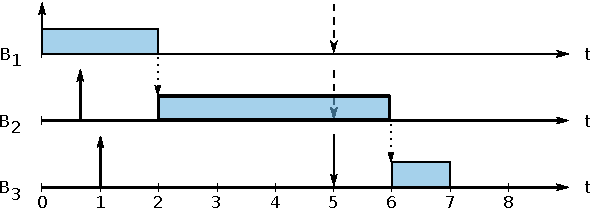
\includegraphics[scale=1.00]{images/producer-worker-consumer}
  \caption{Et generator/arbejder/forbruger -netværk. Kasserne repræsentere det tidsrum hvor processerne bliver bearbejdet. En pil op indikere hvornår processen er klar til at blive eksekveret. En pil ned indikere en deadline for processen. De stiplede pile i proces B$_1$ og B$_2$ til tiden t$=5$ viser en kunstig prioritet på baggrund af B$_3$'s deadline. Den lille stiplede pil mellem  B$_1$ og B$_2$ i t$=2$ og mellem B$_2$ og B$_3$ i t$=6$ viser kommunikation mellem processerne.}
  \label{fig:producer-worker-consumer}
  \end{center}
\end{figure}

\begin{figure}
 \begin{center}
  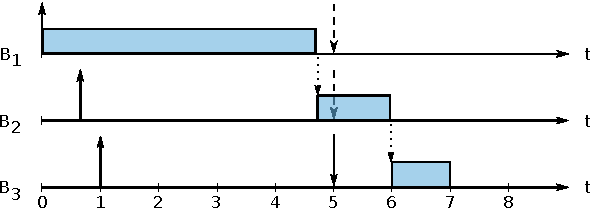
\includegraphics[scale=1.00]{images/producer-worker-consumer2}
  \caption{Samme netværk som i \autoref{fig:producer-worker-consumer}, men i dette tilfælde venter B$_2$  på data fra B$_1$ i hovedparten af tiden inden en deadline.}
  \label{fig:producer-worker-consumer2}
  \end{center}
\end{figure}


Der er dog ikke sikkert at en deadlineException i processer der har nedarvet en prioritet, er med til klarlægge hvilke processer der har brugt alt tiden, og derfor bære skylden for at en deadline ikke blev overholdt. \CRef{fig:producer-worker-consumer2} viser et sådanne eksempel. Netværk er opsat som i \autoref{fig:producer-worker-consumer}, men i dette tilfælde bruger generatorprocessen (B$_1$) alt tiden, og data bliver først sendt fra $B_1$ umiddelbart før en overskridelse af deadlinen. Fra en udvikler  vil det fremgå som var det arbejderprocessen (B$_2$) der er ansvarlig for overskridelsen lige som i \autoref{fig:producer-worker-consumer}, og ikke generatorprocessen $B_1$, som i dette eksempel brugte det meste af tiden. Dermed mister \code{deadlineException} sin troværdighed, og brugbarhed til debugging. I CSP findes desuden begrebet traces, som kan bruges til at se hele forløbet for et program. På nuværende tidspunkt arbejdes der med at introducere traces til \pycsp og når dette er færdigt, vil det være et meget stærkere værktøj til debugging.

Et andet problem ved at kaste en \code{deadlineException} når prioriteterne er overskredet er, at processer måske  ikke er designet til at håndtere en \code{deadlineException}. Udvikleren skal dermed sikrer alle sine processer, hvis ikke hele applikationen skal risikere at stoppe ved en \code{deadlineException}, der ikke bliver håndteret korrekt.  Det er ikke altid en udvikler kan lade processen håndtere en \code{deadlineException}, da begrundelsen for at have introduceret denne oprindelige deadline er kontekstafhængig. og  det er ikke sikkert processen kender denne begrundelse og derfor ikke vil kunne reagere optimalt.

Vi har derfor valgt, at det kun er processer med en eksplicit deadline, der har mulighed for at kaste en \code{deadlineException}. Processer, der nedarver en prioritet, bliver planlagt i henhold til den højeste prioritet, de har, og vil altid  gøre arbejdet færdigt. En proces skal dermed kunne adskille sin egen deadline fra den prioritet, som den skal planlægges med, selv om de to værdier i en stor del af tiden vil være det samme.

En deadline er dermed en variabel der kun kan sættes af udvikleren og det er kun på baggrund af denne deadline at  processen skal kaste en \code{deadlineException}.

For at  \sched en kan udvælge processer introduceres prioritet, der som standard er det samme tal som deadlinen. For at kunne håndtere gentagende prioritetsnedarvning,  gemmes prioriteten i en  liste kaldet \code{inherit\_priotity}. Denne liste af prioriteter  indeholder indledningsvis kun en prioritet som er deadlinen sat af udvikleren. Når andre processer  midlertidigt ønsker at ændre en proces' prioritet, tilføjes den til listen. Ved at bruge en liste i stedet for blot en variabel, har processen mulighed for at blive opprioriteret flere gange og derefter i skridt at vende tilbage til den oprindelige prioritet.

Når \sched en placerer processen i sin hob, bruges blot den mindste prioritet i listen ihht. vores implementering af \sched en. Dette medfører, at når en proces efterfølgende  får ændret sin liste af prioriteter, skal processen genplanlægges for at sikre, at den placeres korrekt i min-hoben i \sched en. 

\subsection{Kanaler}
I \pycsp findes der kun kanaler af type \code{Any-To-Any}, og derfor kan der altid  være et vilkårligt antal kanalender i hver ende af kanalen, der kan være klar til at kommunikere. Vi skal derfor foretage en ændring, så kommunikationen mellem kanalenderne altid foregår mellem de højst prioriterede processer. 

I greenletsversionen foregår udvælgelsen af kanalender til kommunikation ved hjælp af funktionen \code{match}, der udnytter at  hver kanal vedligeholder to lister af processer for hhv. de processer, der ønsker at sende, og modtage data på kanalen. Når en proces eks. ønsker at modtage data, tilføjer den sig selv til listen af processer, der ønsker at modtage, og prøver derefter i \code{match} funktionen at finde en proces, der vil sende data. Er der ingen processer, der venter på at sende data, venter processen på, at en proces melder sig klar til at sende data, ved at kalde \code{match}. Til hver vellykket kommunikation af data vil \code{match} altid blive kaldt to gange, hvor kun den sidste vil resultere i at kommunikationen lykkes.

Ideen bag funktionen \code{match} er enkel og  udnytter, at \code{greenlets}-versionen er enkelttrådet, så hver proces kan løbe listerne igennem, uden andre processer ændre på listernes tilstand.  Vi er kommet frem til, at  en simpel sortering af listerne ud fra processernes interne prioritet vil resultere i, at det altid er den højst prioriterede proces der indgår i kommunikationen. Den ændrede \code{match} kan ses i \cref{lst:match}, hvor det kun er linje 119 og 120 der er ændret.

\begin{lstlisting}[firstnumber=117 ,float=hbtp, label=lst:match, caption=Funktionen \code{match} der sorterer kanalrequests.]
def match(self):        
    if self.readqueue and self.writequeue:
        self.readqueue.sort(key=lambda channelReq:channelReq.process.internal_priority)
        self.writequeue.sort(key=lambda channelReq:channelReq.process.internal_priority)
        for w in self.writequeue:
            for r in self.readqueue:
                if w.offer(r):
                    return       
\end{lstlisting}

Funktionen \code{match} vil blive kaldt en gang for hver proces der ønsker at kommunikere, og derfor vil det kun være det sidste element i listen som ikke er sorteret korrekt ved hver kald af \code{match}. Desuden vil der altid i den ene liste maksimalt være et element der er aktiv, hvorfor den ene liste højst sandsynlig vil være kort, og kørselstiden for de to sorteringer vil derfor være lille. Bemærk desuden at listerne er sorteret så værdien af den interne prioritet er stigende, og derfor er det processen med lavest værdi, der først bliver udvalgt til et match, i overensstemmelse med repræsentationen af prioriteter som nævnt i afsnittet ``Ændringer i \sched en'' \vpageref{sec:sched-changes}.

\subsection{\code{Alternation}}

Som nævnt i afsnit \cref{misc:kanal-prioritet} har vi behov for at kunne tilknytte en prioritet til en kanal for at kunne håndtere udvælgelse i \code{alternations}. Vi har allerede prioriteter for processer og ønsker, at kanalernes prioritet skal defineres på baggrund af hvilke processer, der er tilknyttet kanalen. Vi skal kunne håndtere både input- og output-guards og ønsker seperate prioriteter for disse. Vi tilknytter derfor to prioriteter til hver kanal. De to prioriteter er sat som  de højst prioriterede processer, der er klar til at hhv. modtage og sende data. En kanals prioritet er derfor ikke fast som for processerne, hvor de får sat en prioritet (der dog kan ændres med prioritetsnedarvning), men nærmere en emuleret prioritet, som ændre sig baseret på alle processernes tilstand. 

Til at implementere de to prioriteter introduceres  to hjælpefunktioner, der løber hhv. \code{readqueue} og \code{writequeue} igennem og  finder den højst prioriterede proces, der er villig til hhv. at sende og modtage data. Når  \code{alternation} ønsker at finde prioriteten for en kanal, kigger den på om kanalen i \code{alternation} er tilknyttet en output- eller inputguard og finder den korrekte prioritet.


\subsection{Prioritetsnedarvning}
Prioritet i et RTP system skal ses i forhold til alle processers prioritet. En proces kan derfor ikke i sig selv have en absolut høj prioritet, men kun have høj prioritet ifht. de andre processers prioritet. Ved at give en høj prioritet til  en proces, vil dette dermed  indirekte sænke de andre processers prioritet, et fænomen vi vil kalde ``prioritetsdevaluering``.

For at minimere prioritetsdevaluering i forbindelse med prioritetsnedarvning, ønsker vi at minimere den tid en proces har en kunstigt høj prioritet, og at minimere antallet af processer, hvis prioritet øges. 

Som vi er kommet frem til i \cref{sec:rtp-pycsp-nedarvning}, skal  der foregå  prioritetsnedarvning i forbindelse med kommunikation, hvis der ikke findes nogle processer, der umiddelbart er klar til at kommunikere.  I \pycsp kan man umiddelbart evaluere, om der er processer klar til at kommunikere over en given kanal. Det skyldes, at processer der ønsker kommunikation befinder sig i listerne \code{readqueue} og \code{writequeue}. Hvis ingen processer ønsker at kommunikere, kan man dog ikke finde de processer som potentielt kan indgå i kommunikation.
Vi må derfor udvide kanalerne i RTP versionen med to lister, \code{readerprocesses} og \code{writerprocesses}, der består af de processer, der potentielt kan sende og modtage data over kanalen. Vi håndterer vedligeholdsensen af disse lister, ved at hver proces ved opstart tilføjer sig selv til de kanaler, den har mulighed for at kommunikere over. Et oplagt sted at implementere denne funktionalitet er i processens  \code{\_\_init\_\_}  funktion, da alle kanalender som denne proces potentielt kan kommunikere over, findes som argument til  \code{\_\_init\_\_} funktionen. \CRef{lst:process-init} viser udvidelsen af funktionen, hvor argumenterne gennemløbes, mens der ledes efter kanaler, som processen skal registreres i.

\begin{lstlisting}[firstnumber=29 ,float=hbtp, label=lst:process-init, caption=Uddrag af \code{Process}' \code{\_\_init\_\_}funktion]
for arg in args:
    if isinstance(arg, pycsp.greenlets.channelend.ChannelEndRead):
        arg.channel._addReaderProcess(self)
    if isinstance(arg, pycsp.greenlets.channelend.ChannelEndWrite):
        arg.channel._addWriterProcess(self)  
\end{lstlisting}

Kanaler kender nu  både de processer, der på et specifikt tidspunkt ønsker at kommunikere via listerne \code{readqueue} og \code{writequeue}, og de processer, der potentielt vil kunne kommunikere med listerne \code{readerprocesses} og \code{writerprocesses}. Processer der ønsker at kommunikere kan, som normalt umiddelbart evaluere om det er muligt; såfremt det ikke er muligt, kan den nu evaluere hvilke processers prioritet den kan øge, for at bringe dem i en tilstand hvor de kan indgå i den ønskede kommunikation. 

Funktionaliteten til prioritetsnedarvning skal implementeres i de to interne kommunikationfunktioner  \code{\_read} og \code{\_write}. Fordelen ved at placere prioritetsnedarvning i disse to funktioner er, at de bruges af processerne både i forbindelse med normal blokerende kommunikation og i forbindelse med kommunikation i \code{alternation}. Vi har udvidet funktionerne med følgende liste af begivenheder:
\begin{itemize}
\tightlist
	\item Undersøg om processen opfylder kriterierne for at starte en prioritetsnedarvning.
	\item Forhøj prioriteterne for de potentielle processer i enten \code{readerprocesses} eller \code{writer\-processes}.
	\item Umiddelbart efter kommunikationen nedprioriteres de processer, man midlertidigt har øget prioriteterne på.
\end{itemize}

Som beskrevet er det vigtigt, at vi igennem hele designet forsøger at begrænse mængden af prioritetsnedarvningen, og derfor har vi tilføjet en række egenskaber, der skal være indfriet, før prioritetsnedarvning forsøges. Disse er: processen skal have en prioritet, enten direkte eller efter en nedarvning; kanalen må ikke være klar til kommunikation, hvilket vil sige, at hvis processen ønsker at skrive, må der ikke findes en proces, der er klar til at modtage data; endelige skal processen ikke have overskredet sin egen deadline, da denne til slut blot vil generere en exception, og hele prioritetsnedarvningen vil være irrelevant.

Selve prioritetsforhøjelsen og den senere nedprioritering er simpel, da processen blot sender sin prioritet til alle processerne i den relevante liste dvs. \code{writerprocesses} for  \code{\_read} funktionen og vice versa. Hvis en proces modtagere en lavere prioritet end den endelige prioritet, ses der bort fra hhv. op- og nedjusteringen, så en prioritetsnedarvning ikke resulterer i en forringelse af prioritet. 

